\documentclass[a4paper,11pt]{ltjsarticle}
\usepackage{amsmath, mathtools, mathbbol, amssymb, bm, fancyhdr, anyfontsize, subcaption, multirow, wrapfig, graphicx, hyperref, url, enumitem, ascmac, tikz, tikz-3dplot}
\usetikzlibrary{arrows, angles, quotes}

\hypersetup{
setpagesize=false,
 bookmarksnumbered=true,
 bookmarksopen=true,
 colorlinks=true,
 linkcolor=blue,
 citecolor=black,
 urlcolor=blue,
}

\newcommand{\dlim}[2]{\displaystyle{\lim_{#1 \to #2}\:}}
\newcommand{\dint}[2]{\displaystyle{\int_{#1}^{#2}}}
\def\tick#1#2{\draw[thick] (#1)++(#2:0.12) --++ (#2-180:0.24)}
\def\N{100} % number of samples

\title{高校物理学の解説}
\author{ほうじ茶}
\date{\today}

\begin{document}

\maketitle

\begin{abstract}
  本資料は,高校物理学の解説資料です.高校では,\textbf{微分積分を用いないで}物理基礎や物理を習う.
  その微分積分で得られるの結論を公式として諳記して,問題を解いている.ただし,微分積分なしに物理の問題を解くことは本質的ではない.
  
  本質を1から丁寧に解説し,本質的な理解につなげることを目的とする.
  以下に記載している\textbf{留意事項}をよく読んでから利用のこと.
\end{abstract}

\tableofcontents

\vspace{12pt}

\begin{center}
  \textbf{\color{blue}青文字}をクリックすると,対応したページに遷移します.
\end{center}

\section*{留意事項}

\begin{enumerate}
  \item 色付き文字やハイライトは重要事項または強調箇所です.
  \item 自身の好み(独断と偏見)で作成しているので,旧字体や座標を行列で記載している箇所があります.
  \item 本資料の著作権は,\href{https://creativecommons.org/licenses/by-nc-sa/4.0}{CC BY-NC-SA 4.0}を適応します.
\end{enumerate}

\clearpage

\part{物理学に必要な数学}

\section{スカラーとベクトル}

スカラーは\textbf{1つの数}であり,ベクトルは\textbf{2つ以上の数を束ねたもの}である.
そしてベクトルの表現として\textbf{文字の上に矢印$\vec{x}$を描いて}ベクトルを表現する.ただ,\textbf{非常に見づらく}なりやすいという欠点がある.
そのため,大学以降ではスカラーはそのまま,ベクトルは\textbf{太字}$\bm{x}$または\textbf{2重文字}$\mathbb{x}$(文字に余計な縦線を1つ入れるだけ)で表現する.
よく,スカラーは大きさ\textbf{だけ}持つ量で,ベクトルは大きさと\textbf{向きも}持つ量と理解している人も多い.\colorbox{yellow}{それは何故か?}

\begin{figure}[htbp]
\centering
\begin{minipage}[b]{0.49\columnwidth}
    \centering
    \begin{equation*}
      A = 2
    \end{equation*}
    \caption{スカラー}
\end{minipage}
\begin{minipage}[b]{0.49\columnwidth}
    \centering
    \begin{equation*}
      \bm{B} = (2 \qquad 1 \qquad 3)
    \end{equation*}
    \caption{ベクトル}
\end{minipage}
\end{figure}

スカラーのイメージは,\textbf{1次元}である.すなわち,$x$軸だけの数直線を考えると単なる\textbf{大きさ}にすぎない.
次にベクトルのイメージは,\textbf{2次元}や\textbf{3次元}である.$x$軸だけでは,大きさしか表せなかったのに対し,
数を束にすることで\textbf{2つ目以降の数によって方向が決まる}.

\begin{figure}[htbp]
\centering
\begin{minipage}[b]{0.49\columnwidth}
    \centering
    \begin{tikzpicture}
      \draw[-latex] (-3,0) -- (3,0) node[right]{$x$};
      \foreach \x in {-2,...,2} \draw (\x,0.2)--(\x,0) node[below] {$\x$};
      \draw[->, very thick, cyan] (0,1) -- (2,1);
      \draw[dashed] (0,0) -- (0,1);
      \draw[dashed] (2,0) -- (2,1);
    \end{tikzpicture}
    \caption{スカラー}
\end{minipage}
\begin{minipage}[b]{0.49\columnwidth}
    \centering
    \begin{tikzpicture}
      \draw[-latex] (0,0,0) -- (4,0,0) node[right]{$x$};
      \foreach \x in {1,...,3} \draw (\x,0.2,0)--(\x,0,0) node[below] {$\x$};
      \draw[-latex] (0,0,0) -- (0,4,0) node[above]{$z$};
      \foreach \z in {0,...,3} \draw (0.2,\z,0)--(0,\z,0) node[left] {$\z$};
      \draw[-latex] (0,0,0) -- (0,0,4) node[below]{$y$};
      \foreach \y in {1,...,3} \draw (0.2,0,\y)--(0,0,\y) node[above left] {$\y$};
      \draw[->, very thick, cyan] (0,0,0) -- (2,3,1);
      \draw[dashed] (2,0,0) -- (2,0,1) -- (0,0,1);
      \draw[dashed] (2,3,0) -- (2,3,1) -- (0,3,1) -- (0,3,0) --cycle;
      \draw[dashed] (2,0,0) -- (2,0,1) -- (0,0,1);
      \draw[dashed] (2,0,0) -- (2,3,0);
      \draw[dashed] (2,0,1) -- (2,3,1);
      \draw[dashed] (0,0,1) -- (0,3,1);
    \end{tikzpicture}
    \caption{ベクトル}
\end{minipage}
\end{figure}

\subsection{ベクトルの加減法}

言葉で説明するなら,矢印の終点ともう一方の矢印の始点を合わせ,一つの折れ線矢印と見なし始点と終点を線で結ぶ.減法の場合は,矢印を逆(逆ベクトル)にしてから足す.
ほかに始点同士を揃えて平行四辺形にする方法もあり,運動方程式を解く際の分力を求めるのに最適である.

\hspace{0pt}

\begin{center}
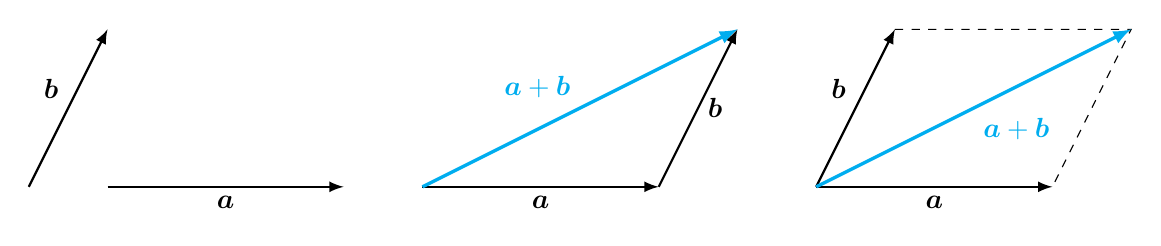
\begin{tikzpicture}
  \draw [-latex,thick] (0,0)--(1,2);
  \node [above left] at ($(0,0)!0.5!(1,2)$) {$\bm{b}$};
  \draw [-latex,thick] (1,0)--(4,0);
  \node [below] at ($(1,0)!0.5!(4,0)$) {$\bm{a}$};
  \draw [-latex,thick] (8,0)--(9,2);
  \node [right] at ($(8,0)!0.5!(9,2)$) {$\bm{b}$};
  \draw [-latex,thick] (5,0)--(8,0);
  \node [below] at ($(5,0)!0.5!(8,0)$) {$\bm{a}$};
  \draw [-latex,very thick,cyan] (5,0)--(9,2);
  \node [above left,cyan] at ($(5,0)!0.5!(9,2)$) {$\bm{a}+\bm{b}$};
  \draw [-latex,thick] (10,0)--(11,2);
  \node [above left] at ($(10,0)!0.5!(11,2)$) {$\bm{b}$};
  \draw [-latex,thick] (10,0)--(13,0);
  \node [below] at ($(10,0)!0.5!(13,0)$) {$\bm{a}$};
  \draw [dashed] (11,2)--(14,2)--(13,0);
  \draw [-latex,very thick,cyan] (10,0)--(14,2);
  \node [below right,cyan] at ($(10,0)!0.5!(14,2)$) {$\bm{a}+\bm{b}$};
\end{tikzpicture}
\end{center}

\vspace{-10pt}

\subsection{単位ベクトル}

ユークリッド空間(実数を$n$個並べた全体の集合)において,3つの直交座標をそれぞれ$x$軸,$y$軸,$z$軸とする.
そのなかで大きさを「1」に仕立てたベクトルを単位ベクトルという.
(単位○○は基本的に,○○の大きさを「1」に仕立てたもののことである.)

また,$x$軸と平行な単位ベクトルを$\bm{i}$,$y$軸と平行な単位ベクトルを$\bm{j}$,$z$軸と平行な単位ベクトルを$\bm{k}$とする.

\subsection{ベクトルの成分表示}

単位ベクトルと係数倍を用いて,一般にベクトルを次のような式で表せる.

\begin{equation}
  \bm{a}=A \bm{i}+B \bm{j}+C \bm{k}
\end{equation}

また,係数を座標のように表して,

\begin{equation}
  \bm{a}=(A \quad B \quad C)
\end{equation}

とも表せる.

\clearpage

\part{電磁気}

\section{電気はスカラー,磁気はベクトル}

\subsection{スカラーとベクトルの復習}

スカラーとベクトルの違いは,力学でも扱った.スカラーは\textbf{1つの数}であり,ベクトルは\textbf{2つ以上の数を束ねたもの}であった.
そして,スカラーはそのままでいいが,ベクトルは\textbf{太字}または\textbf{2重文字}で表現する.
よく,スカラーは大きさ\textbf{だけ}持つ量で,ベクトルは大きさと\textbf{向きも}持つ量と理解している人も多い.\colorbox{yellow}{それは何故か?}

\begin{figure}[htbp]
\centering
\begin{minipage}[b]{0.49\columnwidth}
    \centering
    \begin{equation*}
      A = 2
    \end{equation*}
    \caption{スカラー}
\end{minipage}
\begin{minipage}[b]{0.49\columnwidth}
    \centering
    \begin{equation*}
      \bm{B} = (2 \qquad 1 \qquad 3)
    \end{equation*}
    \caption{ベクトル}
\end{minipage}
\end{figure}

スカラーのイメージは,\textbf{1次元}である.すなわち,$x$軸だけの数直線を考えると単なる\textbf{大きさ}にすぎない.
次にベクトルのイメージは,\textbf{2次元}や\textbf{3次元}である.$x$軸だけでは,大きさしか表せなかったのに対し,
数を束にすることで\textbf{2つ目以降の数によって方向が決まる}.

\begin{figure}[htbp]
\centering
\begin{minipage}[b]{0.49\columnwidth}
    \centering
    \begin{tikzpicture}
      \draw[-latex] (-3,0) -- (3,0) node[right]{$x$};
      \foreach \x in {-2,...,2} \draw (\x,0.2)--(\x,0) node[below] {$\x$};
      \draw[->, very thick, cyan] (0,1) -- (2,1);
      \draw[dashed] (0,0) -- (0,1);
      \draw[dashed] (2,0) -- (2,1);
    \end{tikzpicture}
    \caption{スカラー}
\end{minipage}
\begin{minipage}[b]{0.49\columnwidth}
    \centering
    \begin{tikzpicture}
      \draw[-latex] (0,0,0) -- (4,0,0) node[right]{$x$};
      \foreach \x in {1,...,3} \draw (\x,0.2,0)--(\x,0,0) node[below] {$\x$};
      \draw[-latex] (0,0,0) -- (0,4,0) node[above]{$z$};
      \foreach \z in {0,...,3} \draw (0.2,\z,0)--(0,\z,0) node[left] {$\z$};
      \draw[-latex] (0,0,0) -- (0,0,4) node[below]{$y$};
      \foreach \y in {1,...,3} \draw (0.2,0,\y)--(0,0,\y) node[above left] {$\y$};
      \draw[->, very thick, cyan] (0,0,0) -- (2,3,1);
      \draw[dashed] (2,0,0) -- (2,0,1) -- (0,0,1);
      \draw[dashed] (2,3,0) -- (2,3,1) -- (0,3,1) -- (0,3,0) --cycle;
      \draw[dashed] (2,0,0) -- (2,0,1) -- (0,0,1);
      \draw[dashed] (2,0,0) -- (2,3,0);
      \draw[dashed] (2,0,1) -- (2,3,1);
      \draw[dashed] (0,0,1) -- (0,3,1);
    \end{tikzpicture}
    \caption{ベクトル}
\end{minipage}
\end{figure}

電気は導線上に流れるので,大きさだけを考えて「オームの法則」や「キルヒホッフの法則」は計算できる.
一方で磁気はどうだろうか?何かの軌道に乗っている訳ではない.磁石を思い浮かべると,どんな場所からでも引力や斥力の影響を受ける.
このような環境のことを一般に\textbf{場}と呼ぶ.

\subsection{点から線,束そして場へ}

この話は簡単である.点が複数集まることで線になる.線が複数集まることで束になる.そして,束が場を作り出すということだ.

\end{document}